\section{Proposed Work }
For this project, I propose and implement a NMT system that is able to handle rare and unknown words in an unsupervised fashion and study the effectiveness of the technique. This involves analyzing words for their morphology and getting good vector representation for word based its morphological components. This project requires implementing two major systems.

\begin{itemize}
	\item Implementing an NMT system with encoder-decoder architecture.
	\item Implementing an morphological analyzer to handle rare and unknown words in an online fashion.
\end{itemize}


For NMT system, I will implement the attention based encoder-decoder RNN model from \cite{bahdanau2014neural}. They use a soft attention model that determines which words to focus in source language while generating target language words. For morphological analyser, I will extend the work of \cite{soricut2015unsupervised} where they proposed an language-agnostic, unsupervised method for inducing morphological transformation between words. Although the technique was proposed for lexicon generation, the morphological rules and their vector representations learned by the technique can be used to produce vector representations for OOV words in NMT systems. These two systems are explained in detail in the section below.




\subsection{Attention based Encoder-Decoder model \citep{bahdanau2014neural}}

\cite{bahdanau2014neural} proposed an attention based encoder-decoder architecture which is capable of learning word alignment between source and target sentences. This allowed for the encoder to produce better sentence representation for longer sentence which in turn improved the translation quality. In their additive approach, a single feed forward neural networks that can learn to assign different weights to the hidden layer vectors was used. These weighted sum of the hidden layer vectors $h_{1:n}$ called context vectors $c_i$ is calculated each time decoder generates a new word as shown in figure \ref{attention}.


\begin{align*}
c_i &= \sum_{j=1}^{n} \alpha_{ij} h_j \\
\alpha_{ij} &= \frac{\hat{a}_{ij}}{\sum_j \hat{a}_{ij}}\\
\hat{a}_{ij} &= att(s_i, h_j)
\end{align*}

where $att(s_i, h_j)$ is an attention function that calculates the weights for each encoder hidden state $h_{1:n}$ for a given decoder state $s_i$. \cite{bahdanau2014neural} also used bi-directional RNN which reads the sentence from both directions. The state vector from both direction right to left  $\overleftarrow{h_i}$ and left to right $\overrightarrow{h_i}$ is concatenated for each word. The attention mechanism is applied over this concatenated hidden state vector $h_i = [\overleftarrow{h_i};\overrightarrow{h_i}]$. The whole network is trained with negative log-likelihood as objective function using stochastic gradient descent.


\begin{figure}[ht]
	\centering
	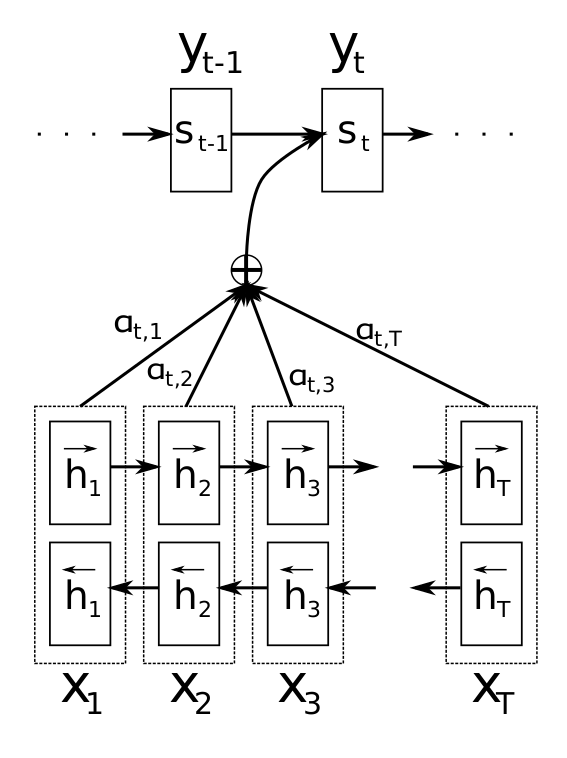
\includegraphics[scale=0.4]{images/attention}
	\caption{Attention based encoder \citep{bahdanau2014neural}}.
	\label{attention}
\end{figure}

\subsection{Unsupervised Morphological induction \citep{soricut2015unsupervised}}

\cite{soricut2015unsupervised} proposed a language-agnostic, heuristic method to capture morphological transformations by exploiting regularities present in word embeddings \citep{mikolov2013distributed}. Their method automatically induces morphological rules and transformations to represent them as vectors in the same embedding space. During testing, out of vocabulary words can be mapped into the same vector space using the learned morphological transformations. In this algorithm, the morphological rules are learned as follows.

\begin{enumerate}
	\item Extract candidate morphological rules like \textit{('suffix', 'ies', 'y')} (replace suffix \textit{ies} with \textit{y}) from word pairs in vocabulary V and evaluate their quality in the pre-trained embedding space.
	\item Generate morphological transformation from the above candidate rules and build a cyclic, multi-graph representing words as nodes and edges as morphological transformations.
	\item Build a normalized acyclic graph (based on word frequency) with 1-1 morphological mapping from the above graph.
	\item Map the rare/out of vocabulary words in the same vector space using morphological transformation using the graph.
\end{enumerate}

Using this approach, if the word \textit{unassertiveness} occurs in the source sentence and is not found the vocabulary of the word embedding, we would be able to get a reasonably good vector representation for the word. Traditionally, any word not in vocabulary is mapped to \textit{unk}. Using the approach from  \cite{soricut2015unsupervised}, we will be able to learn vector representation for morphological transformations like \textit{(prefix,un,$\epsilon$)} and \textit{(suffix,$\epsilon$,ness)}. Then, these morphological rules and their vector representation can be used to map the OOV word \textit{unassertiveness} to  \textit{assertive} and get a good vector representation. 

